\newpage
\appendix
\chapter{Apêndice}
\section{Questionário de Perfil do Usuário}

	Este questionário foi utilizado para identificar o perfil do usuário e algumas de suas necessidades. 




\begin{figure}[h]
    \centering
    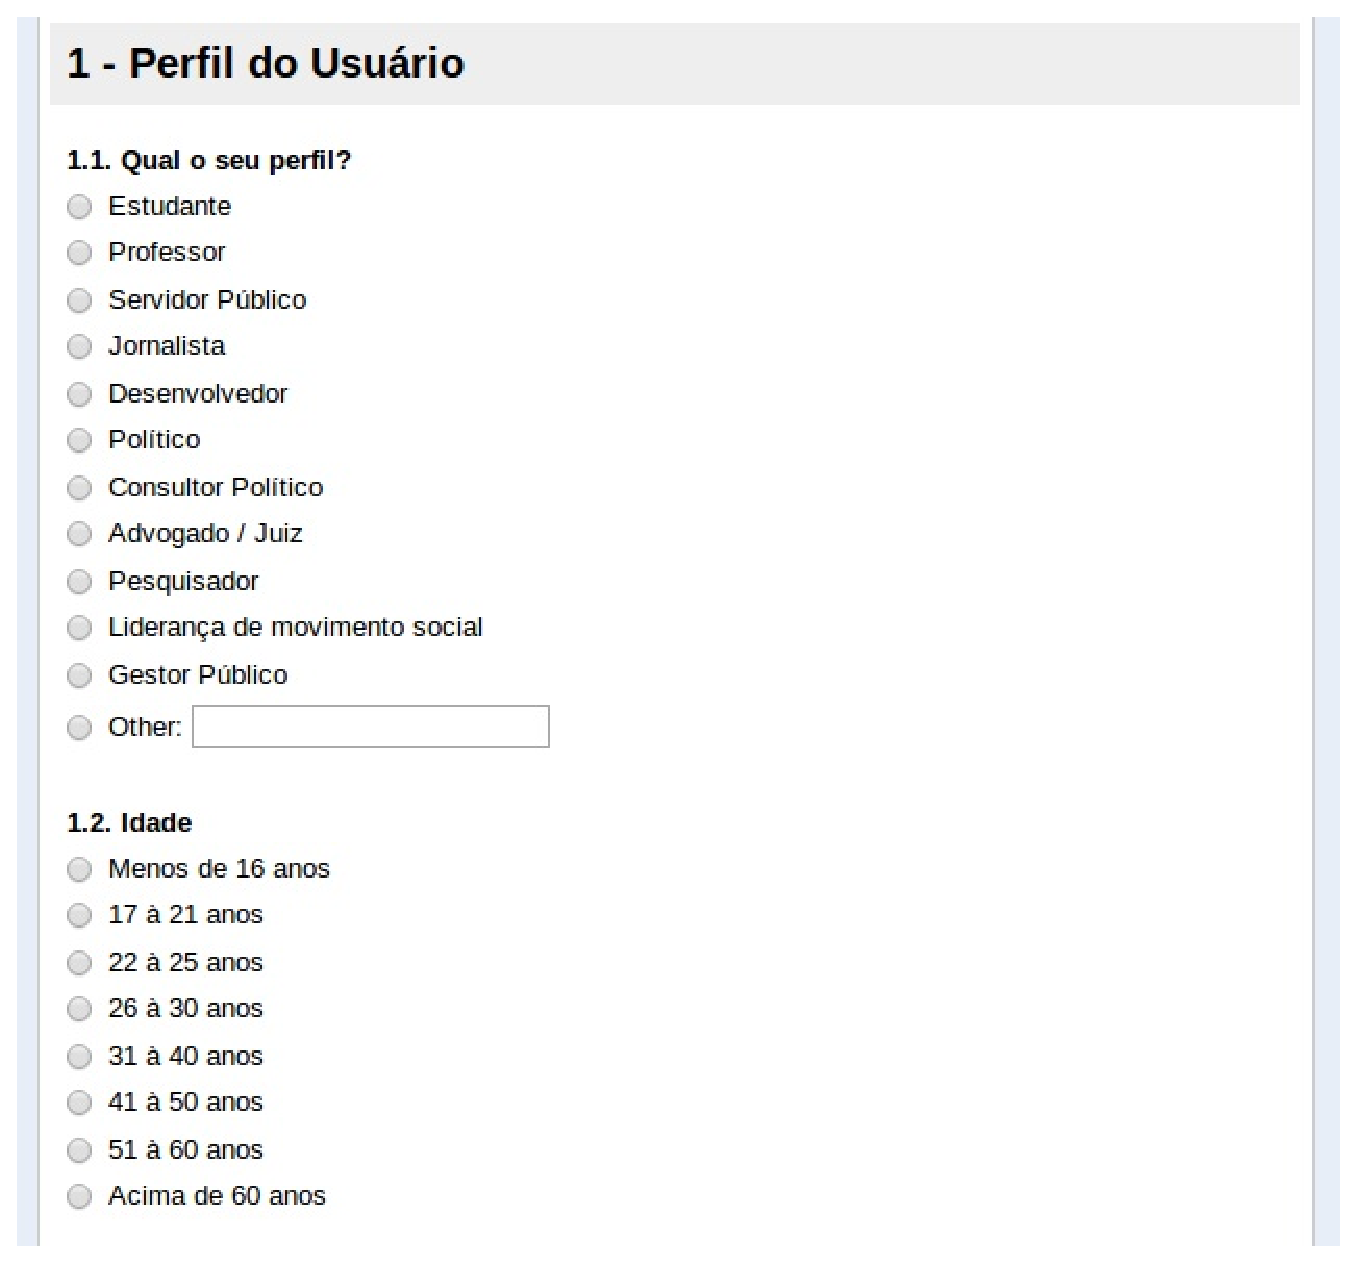
\includegraphics[keepaspectratio=true,scale=0.60]
      {figuras/perf1.eps}
	\caption{Questionário de perfil do usuário}
    \label{perfilgeral}
\end{figure}
%
%
\newpage


A primeira parte do questionário mostra perguntas gerais referentes ao perfil social dos usuários como idade, ocupação/profissão, gênero, formação adadêmica e áreas de interesse.



\begin{figure}[!h]
    \centering
    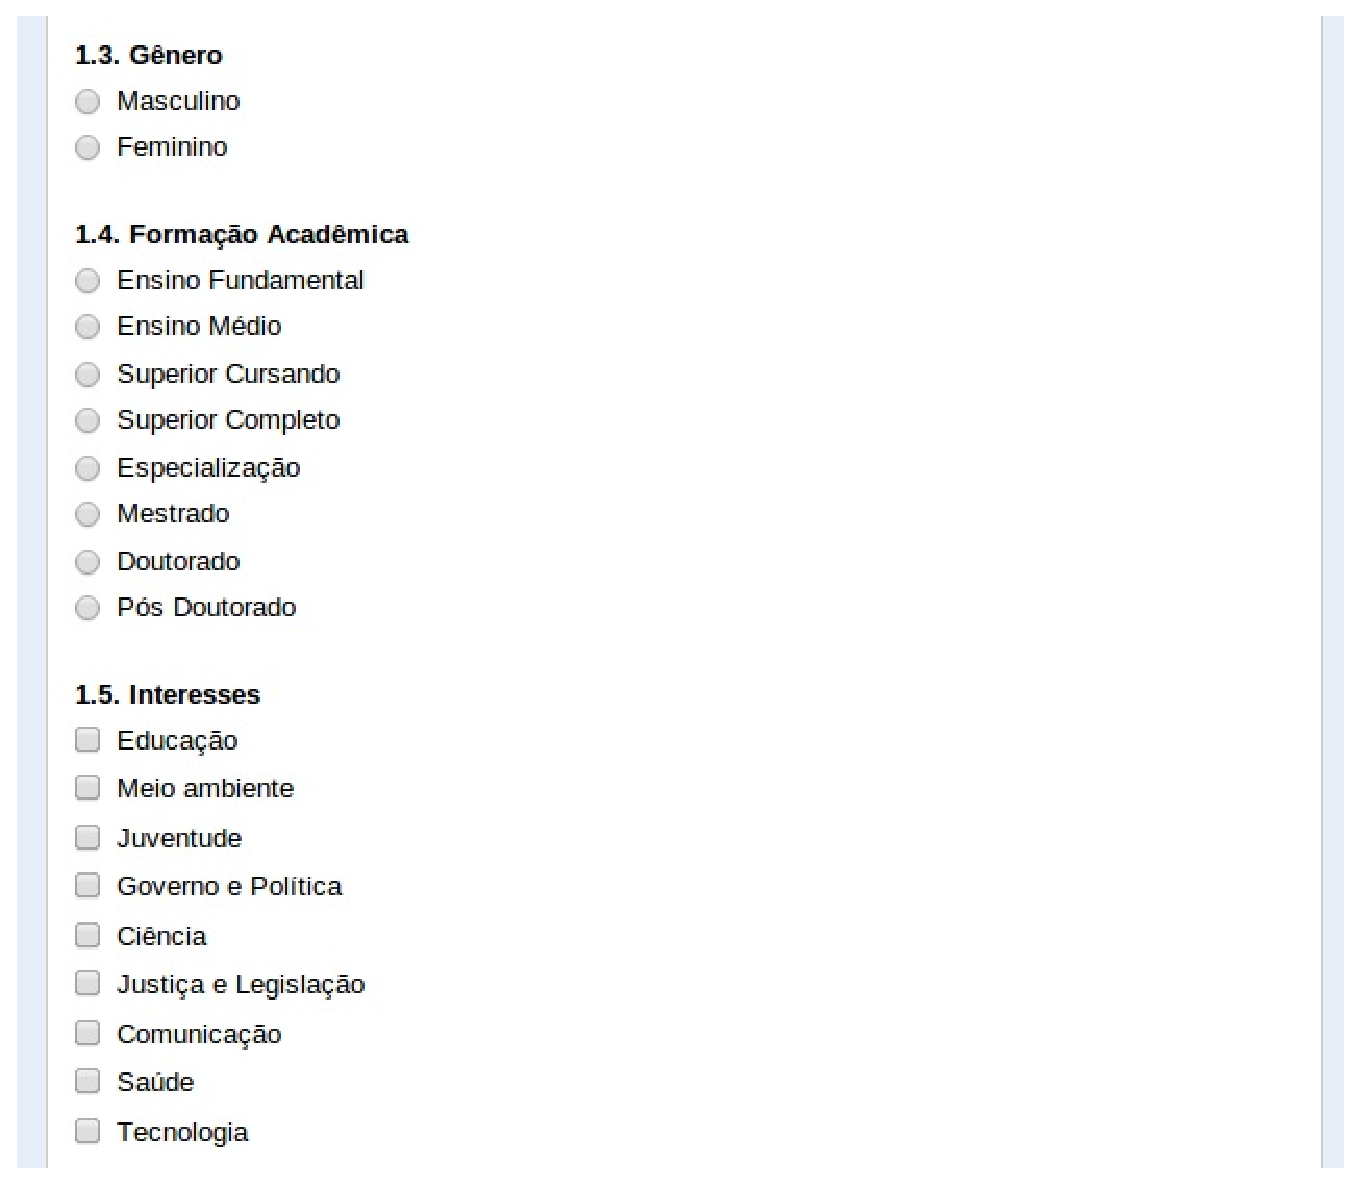
\includegraphics[keepaspectratio=true,scale=0.60]
      {figuras/perf2.eps}
     \caption{Questionário de perfil do usuário - Continuação}
    \label{perfilgeral}
\end{figure}
	
\newpage

	Na seção dois do questionário, as informações sobre o uso dos meios de comunicação que cada usuário. Informações sobre locais de acesso à internet, velocidade de conexão, principais redes sociais e as principais atividades que realiza na internet. 


\begin{figure}[!h]
    \centering
    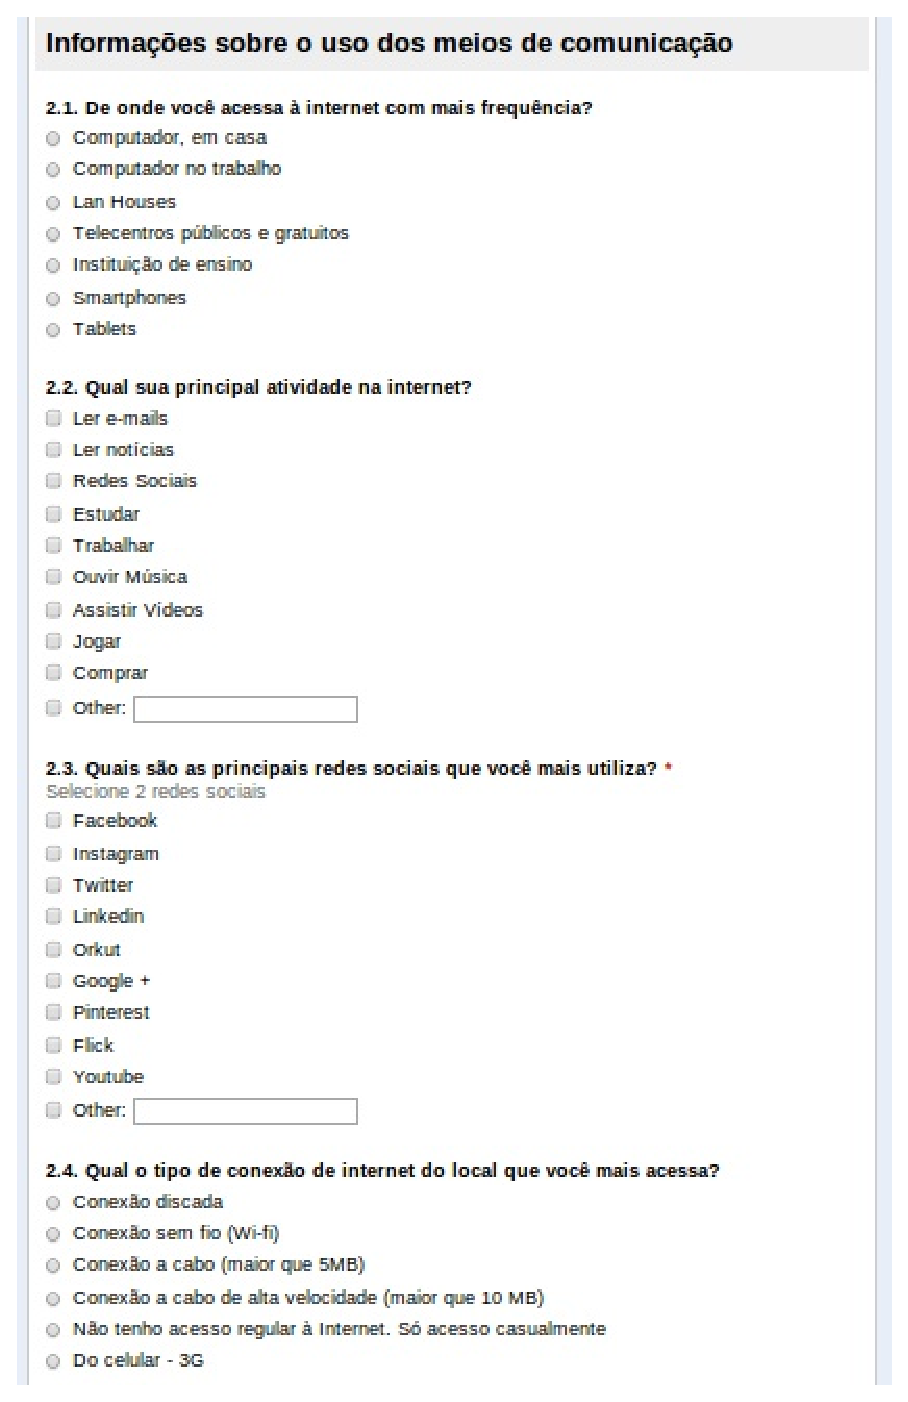
\includegraphics[keepaspectratio=true,scale=0.60]
      {figuras/perf03.eps}
    \label{meiosdecomunicaçaõ}
	\caption{Informações sobre o uso dos meios de comunicação}
\end{figure}

\newpage


	Na terceira seção do questionário são feitas perguntas referentes ao engajamento político/social dos usuários como atuações em movimentos políticos e sociais e participações em manifestações, além de saber sobre o meio de informação na qual se informa sobre os movimentos.





\begin{figure}[!h]
    \centering
    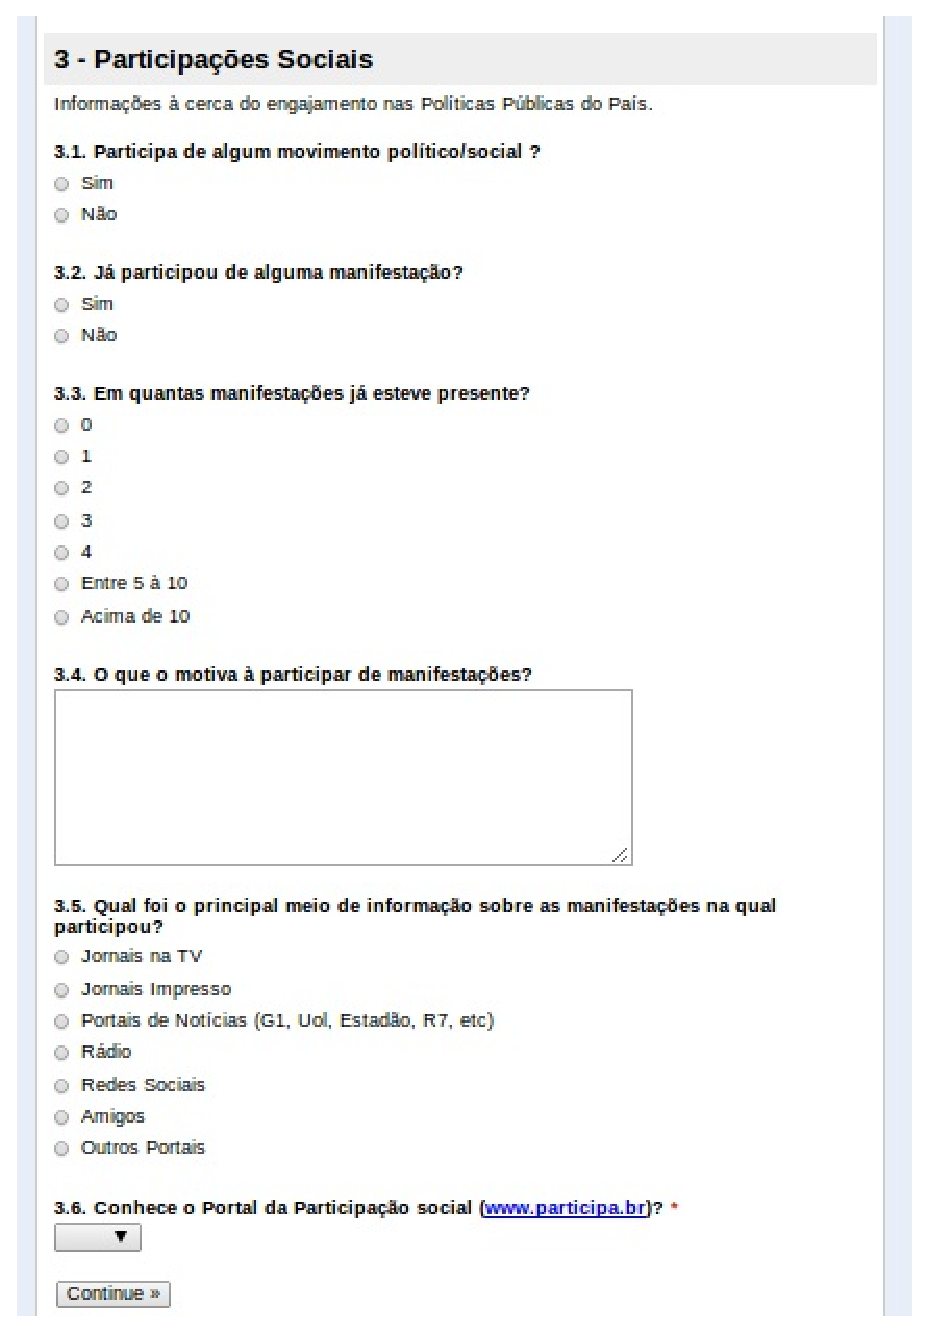
\includegraphics[keepaspectratio=true,scale=0.60]
      {figuras/perf4.eps}
    \caption{Participações sociais}
    \label{participações}
\end{figure}

\newpage

	Depois que foram preenchidas a primeira parte do questionário, os usuários que já usavam o portal da participação social iriam preencher algumas outras questões referente a utilização do portal, tentando entender as principais atividades e funcionalidades que cada usuário utilizava.




\begin{figure}[!h]
    \centering
    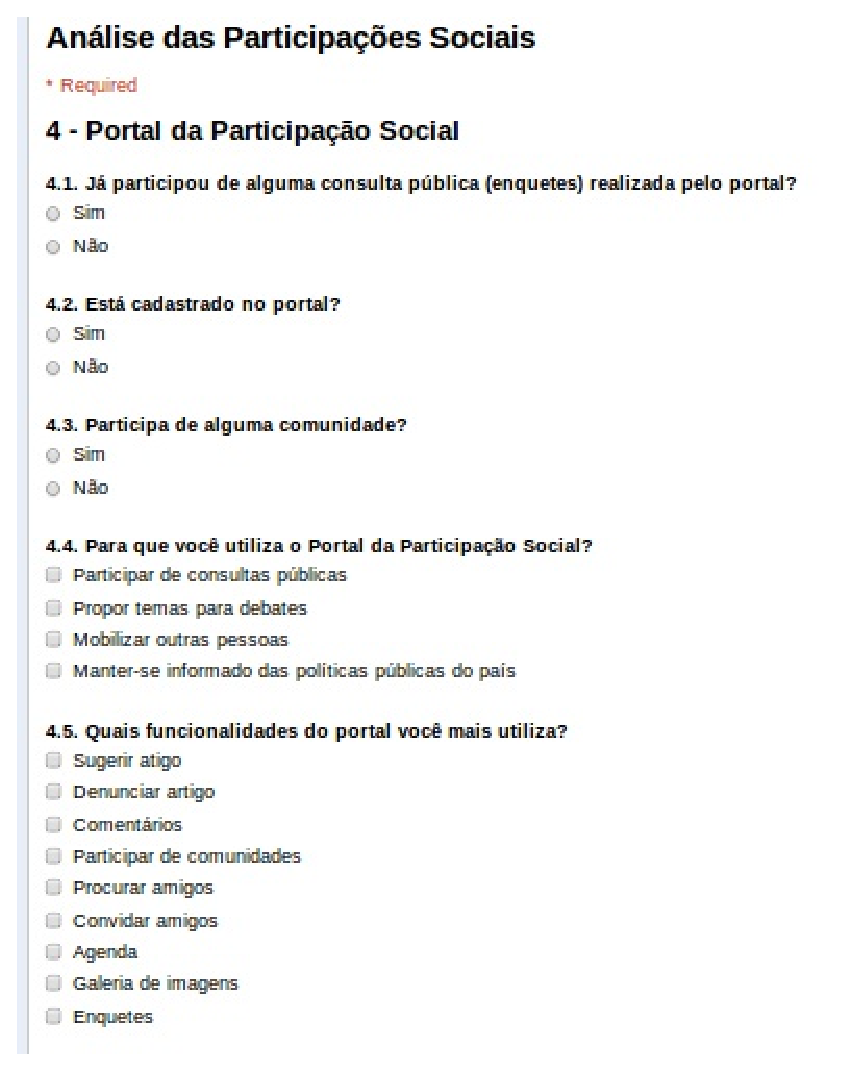
\includegraphics[keepaspectratio=true,scale=0.60]
      {figuras/perf5.eps}
    \caption{Portal da Participação Social}
    \label{participabr}
\end{figure}


\newpage

	Na seção cinco do questionário, as questões servem para conhecer o tempo e o local de acesso dos usuários do portal da participação social




\begin{figure}[!h]
    \centering
    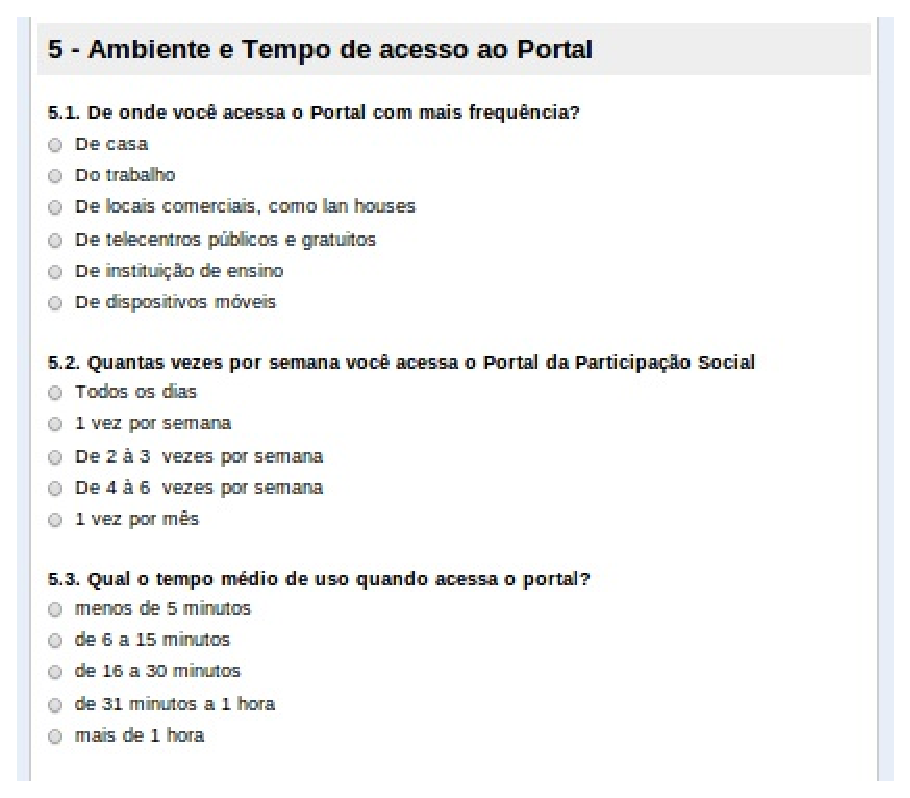
\includegraphics[keepaspectratio=true,scale=0.60]
      {figuras/perf6.eps}
    \caption{Ambiente e tempo de acesso no portal}
    \label{acessoportal}
\end{figure}


\section{Questionário de Satisfação}

	Levantamos informações sobre alguns questionários de satisfação de uso existentes na literatura e foi feito uma comparação entre cada um deles.

\subsection{QUIS - Questionnaire for User Interaction Satisfaction}

	O QUIS mede a satisfação do usuário quanto â usabilidade do produto de maneira padronizada, segura e válida, a fim de obter informações precisas em relação à reação dos usuários a novos produtos (QUIS, 2009);

	A versão atual é a QUIS 7.0 (Norman e Shneiderman, 2010), contém um questionário onde possui a avaliação da satisfação geral e avaliações de fatores específicos de interfaces organizadas hierarquicamente: tela, terminologia e retroalimentação do sistema, aprendizado, capacidades do sistema, manuais técnicos, tutoriais online, multimídia, teleconferência e instalação de software. Pode ser configurado de acordo com a necessidade e interesse do usuário. 

	É um questionário proprietário, é sugerido o uso de planilhas eletrônicas e softwares estatísticos até que se implementem recursos de análise no servidor web dos proprietários.

\subsection{SUS – System Usability Scale}

	O SUS é uma escala de usabilidade do tipo Likert que possui uma visão global e subjetiva em suas avaliações de usabilidade. Ele apresenta ao entrevistado uma lista de perguntas que devem ser respondidas em uma escala de satisfação (indica o grau de concordância ou discordância do usuário) \cite{brooke1996sus}.

	O autor se baseou na afirmação de que no contexto industrial, as avaliações completas não são práticas e requerem muito esforço e custo. O SUS foi criado pela necessidade de se ter uma avaliação de usabilidade simples e rápida. Os métodos de avaliação foram simplificados e o número de questões reduzidas, pois uma quantidade grande de questões desanima os usuários que possivelmente não preencheria todas as questões, resultando assim problemas na captura de reações subjetivas do usuário. Foi então proposto um questionário com 10 questões que utiliza a escala Likert de cinco ou sete pontos. Este questionário abrange vários aspectos da usabilidade, tais como: necessidade de suporte, treinamento e complexidade. ~\cite{preece2007}

\subsection{SUMI – Usability Measurement Inventory}

	O SUMI proposto por ~\citeonline{kirakowski1988measuring} é um questionário para medição da qualidade de um software do ponto de vista do usuário, é um método consistente usado para avaliar a qualidade de uso de um produto de software ou protótipo, e pode ajudar na descoberta de falhas de usabilidade. É mencionado na norma ISO 9241 como um método reconhecido para testar a satisfação do usuário. O SUMI é um questionário comercial. 

	Inicialmente continha 150 itens onde o participante escolhia se (concordo fortemente, concordo, não sei, discordo ou discordo totalmente). Atualmente são 50 itens divididos em 5 grupos de 10 itens. Os grupos de itens são: eficiência, afeto, eficácia, controle e aprendizado. Os entrevistados preenchem o questionário no seu local de trabalho e devem decidir entre as opções: concordo, não sei ou discordo totalmente.

\subsection{ASQ – The After-Scenario Questionnaire}

O ASQ é um questionário de três itens que são utilizados para avaliar a satisfação do usuário após a conclusão de cada cenário/tarefa. São realizadas umas séries de tarefas que estão de acordo com a realidade do usuário.Este questionário aborda questões como: facilidade de conclusão da tarefa, tempo para completar uma tarefa e adequação das informações de suporte.São questões do tipo Likert, aplicando uma escala de 1 a 7, onde 1 representa “Concordo totalmente” e 7 para “Discordo totalmente”. ~\cite{lewis1995ibm}

O participante gasta em média 1 hora pra realizar cada cenário, no fim de cada cenário é preenchido o questionário ASQ. Após completar todos os cenários, no fim de 1 dia de trabalho (8 horas), os participantes preenchem o questionário PSSUQ para avaliação geral do sistema.O ASQ foi aplicado na IBM por diferentes tipos de usuários, cada grupo possuía um tempo de experiência com sistemas de computador, o que permitiu a análise psicométrica do questionário.

\begin{figure}[!h]
    \centering
    \includegraphics[keepaspectratio=true,scale=0.60]
      {figuras/asq.eps}
    \label{ASQ - The After-Scenario Questionnaire }
	\caption{ASQ - The After-Scenario Questionnaire}
\end{figure}

\subsection{PSQ – The Printer-Scenario Questionnaire}

O PSQ  é uma versão inicial do ASQ, mas difere no formato e numero de itens.  São escalas de 5 pontos com os termos “Aceitável” com nota 1 e “Precisa de muita Melhoria” com nota 5, e não marcado “Para Avaliar” ~\cite{lewis1995ibm}.

\subsection{PSSUQ – The Post-Study System Questionnaire}

	O PSSUQ fornece uma avaliação global do sistema utilizado. Esse questionário possui 19 itens para avaliação da satisfação do usuário com a usabilidade do sistema. É gasto em média 10 minutos para completar o questionário, mas só é preciso completar uma vez o questionário no fim do estudo de usabilidade. ~\cite{lewis1995ibm} 

	Este questionário ajuda a entender quais aspectos do sistema o usuário está mais preocupado. Ele avalia as características como facilidade de uso e de aprendizado, simplicidade, eficácia, informação e a interface com o usuário.

	Existem 4 tipos de pontuações para as respostas aos itens do PSSUQ: Escore da satisfação geral (OVERALL), a utilidade do sistema(SYSUSE), a qualidade da  informação (INFOQUAL) e a qualidade da interface (INTERQUAL). 

A escala Global está relacionada com a soma das classificações ASQ que os participantes deram após completar cada cenário. 

%fonte lewis2002psychometric

\begin{figure}[!h]
    \centering
    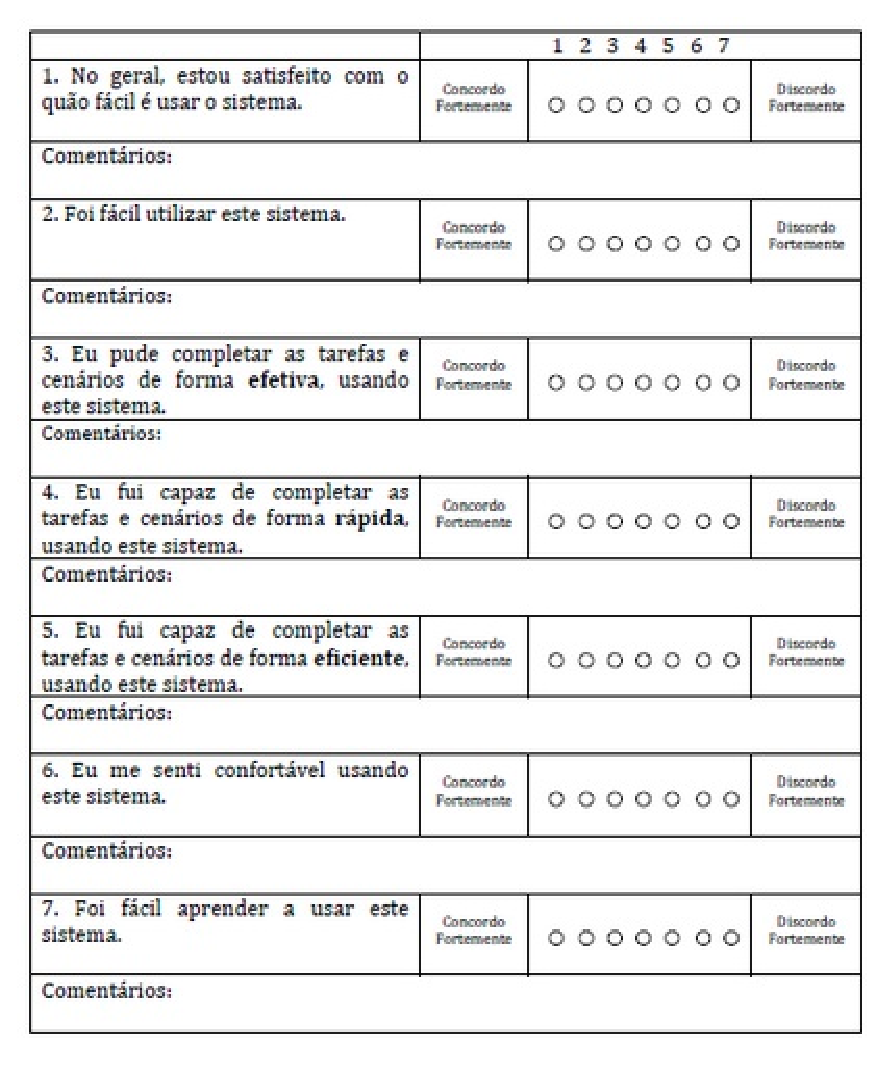
\includegraphics[keepaspectratio=true,scale=0.60]
      {figuras/pssuq01.eps}
    \label{pssuq}
	\caption{PSSUQ – The Post-Study System Questionnaire}
\end{figure}

\newpage

\begin{figure}[!h]
    \centering
    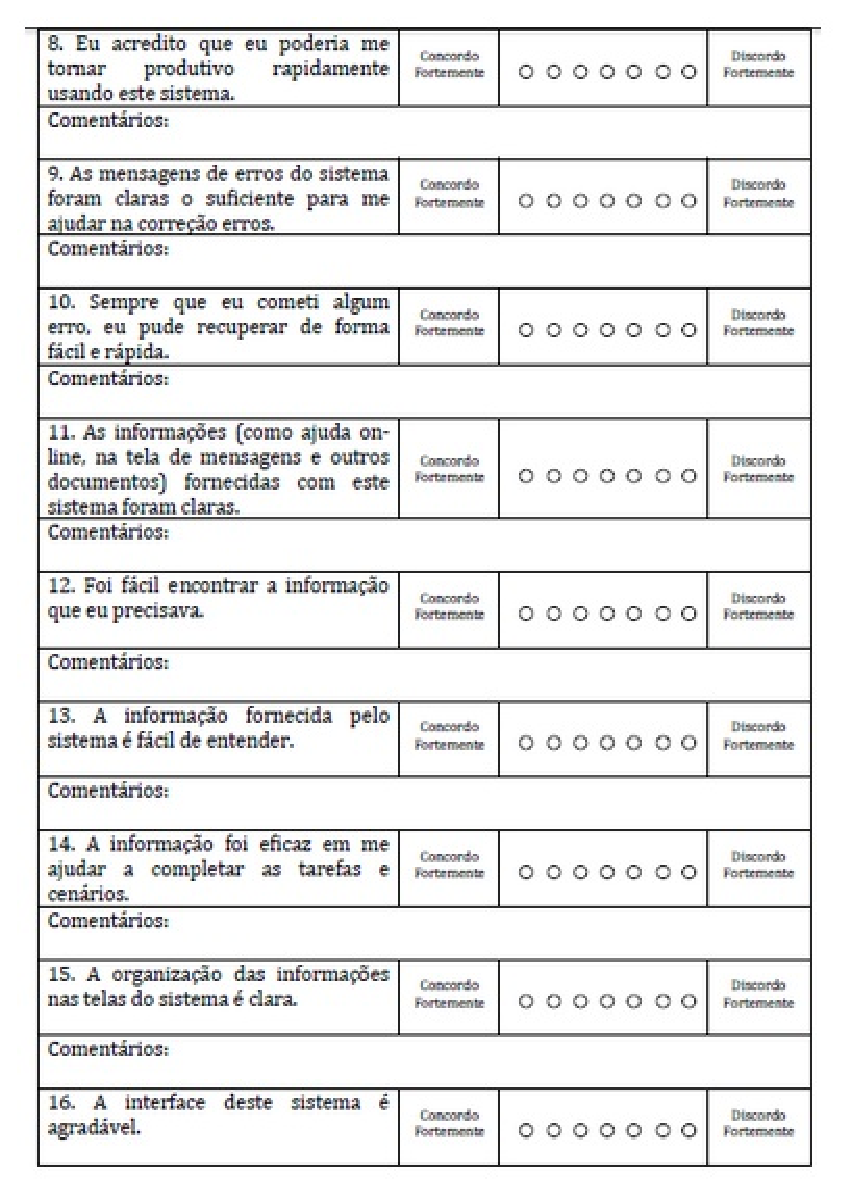
\includegraphics[keepaspectratio=true,scale=0.60]
      {figuras/pssuq02.eps}
    \label{pssuq}
\end{figure}

\begin{figure}[!h]
    \centering
    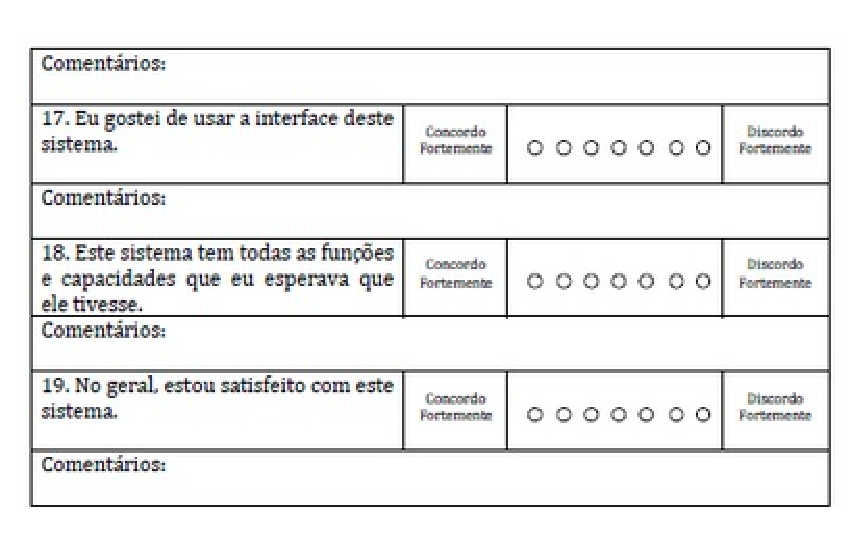
\includegraphics[keepaspectratio=true,scale=0.60]
      {figuras/pssuq03.eps}
    \label{pssuq}
	\caption{PSSUQ: The Post-Study System Questionnaire - Questões de 8 à 19}
\end{figure}

\subsection{CSUQ - Computer System Usability Questionnaire}

	Este questionário é parecido com o PSSUQ, mas a sua redação e diferente. Enquanto no PSSUQ afirma que “Eu poderia efetivamente realizar as tarefas e cenários usando este sistema” o CSUQ escreve: “Eu posso terminar meu trabalho de forma eficaz usando esse sistema?”. Na IBM, este questionário foi aplicado através de e-mail, enviado para funcionários de diferentes locais, o que houve uma maior quantidade de participantes, do que feito com grupos reduzidos presencialmente. ~\cite{lewis1995ibm} 
	O CSUQ é utilizado quando o estudo de usabilidade é em um ambiente fora do laboratório. A confiabilidade relatada foi de 0,93.



\subsection{Comparativo dos questionários}

	Os questionários ASQ e PSQ são utilizados após a realização de um cenário. Contém os mesmos itens, mas possuem escalas diferentes. O ASQ possui uma maior confiabilidade em relação ao PSQ. 

	PSSUQ e CSUQ são ambos os questionários de satisfação global. O PSSUQ utiliza itens adequados para uma situação de teste de usabilidade, já o CSUQ são apropriados para uma situação de teste de campo. Os questionários possuem propriedades psicométricas aceitáveis de usabilidade e podem ser usados com confiança como medidas padronizadas de satisfação. É interessante utilizar o PSSUQ junto com o ASQ.

	O ideal é que o questionário seja mais genérico possível. Cada questionário possui um nível de confiança.

\begin{table}[h]
\begin{tabular}{l|l|l|l|p{3cm}|l|l|}
\hline
\textbf{Nome} & \textbf{Criador} & \textbf{Questões} & \textbf{Licença} & \begin{tabular}[c]{@{}l@{}}\textbf{Interface  Avaliada}\end{tabular}  & \textbf{Confiab.} & \textbf{Escala} \\ \hline
ASQ & IBM & 3 & Aberto & Qualquer & 0,93 & \begin{tabular}[c]{@{}l@{}}Discordo \\ Fortemente /\\ Concordo \\ Fortemente\end{tabular} \\ \hline
\begin{tabular}[c]{@{}l@{}}CSUQ\end{tabular}    & IBM              & 19       & Aberto          & \begin{tabular}[c]{@{}l@{}}Baseado em\\ computador \end{tabular} & 0,95           & \begin{tabular}[c]{@{}l@{}}Discordo \\Fortemente /\\ Concordo \\ Fortemente\end{tabular} \\ \hline
\begin{tabular}[c]{@{}l@{}}PSSUQ\end{tabular} & IBM              & 19       & Aberto          & \begin{tabular}[c]{@{}l@{}}Baseado em\\ computador \end{tabular} & 0,96           & \begin{tabular}[c]{@{}l@{}}Discordo \\ Fortemente /\\ Concordo\\ Fortemente\end{tabular} \\ \hline
\begin{tabular}[c]{@{}l@{}}SUMI\end{tabular}   & HERG             & 27       & Proprietário    & Software              & 0,89           & \begin{tabular}[c]{@{}l@{}}Discordo \\Fortemente /\\ Concordo\\ Fortemente\end{tabular} \\ \hline
SUS                                                                 & DEC              & 10       & Aberto          & Qualquer              & 0,85           & \begin{tabular}[c]{@{}l@{}}Discordo \\Fortemente / \\Concordo \\Fortemente    \end{tabular}                                         \\ \hline
QUIS                                                                                         & UMD              & 50       & Proprietário    &       -         &       -         & 0 a 9                                                                               \\ \hline
\end{tabular}
\caption {Comparativo dos questionários}
\end{table}

 
\section{Cenários}

	Os cenários foram levantados através de uma análise do que era permitido de realizar no portal e quais seriam mais importantes para as principais atividades de um usuário.

	Através das redes sociais e do perfil do usuário no portal da participação social foi identificado que uma das atividades mais realizadas pelos usuários são de edição de textos no blog do perfil, além da criação de mecanismos de participação social como a votação em pares (parwise).
	
	Entender o perfil do usuário é um dos principais pontos que devem ser levados em consideração pelos desenvolvedores de software em geral. Cada perfil de usuário tem suas particularidades e suas expectativas quanto a utilização do sistema.

